\section{Utilisation du logiciel}
\subparagraph{}
Au cours de l'avancement du projet, nous avons choisi un juste milieu entre la quantit\'e de d\'eveloppement de l'interface graphique et les fonctionnalit\'es d'analyse du graphe. Ambitieux, nous souhaitions pousser l'analyse loin et réaliser une interface graphique évoluée.

\subsection{Fonctionnement global}
\subparagraph{}
Le logiciel fonctionne \`a partir de fichiers de données recensant la topologie d'internet et sa structure. Il doit permettre entre autre de construire un graphe et de permettre son affichage dans une fenêtre en Qt.

Rappelons que le voeu de l'application est d'utiliser les structures de donn\'ees \textit{Boost} et que nous avons adopté le pattern MVC afin de développer de manière plus ind\'ependante l'interface graphique du coeur de l'application. La pi\`ece centrale de ce système est la communication entre le modèle et la vue, en d'autres termes : le contrôleur. Voici la liste de ses fonctionnalités :
\begin{itemize}
 \item lancer la lecture des fichiers de données afin de construire le graphe,
\item obtenir le nombre d'AS, de liens, et d'autres informations globales sur le graphe,
\item récupérer le graphe sans les stubs,
\item récupérer l'adjacence d'un AS,
\item récupérer les informations concernant un AS (centrality, numéro),
\item ne récupérer qu'une partie du graphe en fonction de la centralité des sommets,
\item calculer les coordonnées que les sommets doivent avoir sur l'interface graphique.
\end{itemize}

L'ensemble de ces fonctionnalités se retrouve dans l'interface graphique, qui sera présentée ci-dessous.

%ATTENTION : \'ebauche pour cette partie.
\subsection{Description du programme}
\subparagraph{}
Le programme tel que le voit l'utilisateur est une fen\^etre graphique avec un menu en haut, une zone d'affichage au centre, et une zone de notification en bas.

\begin{figure}[H]
\centering
 \fbox
 {
 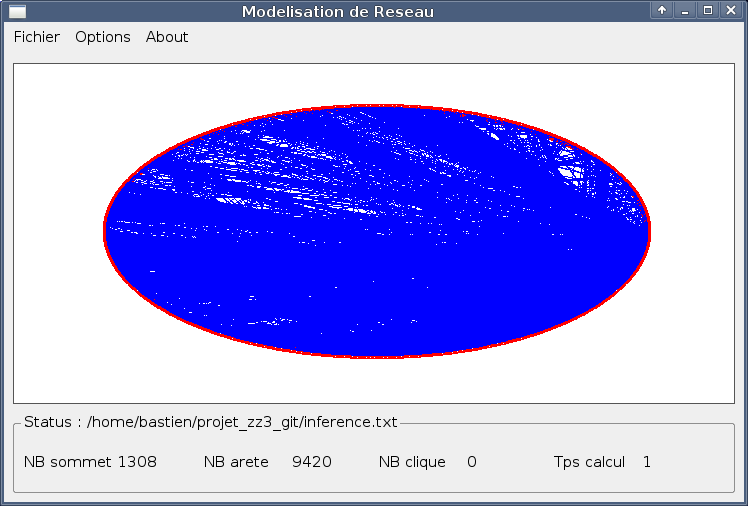
\includegraphics[width=16cm]{./schema/capture_ecran_programme.png}
 }
  \caption{\label{ecran_principal}Ecran principal du programme}
\end{figure}


Le menu comporte trois types d'entr\'ees :
\begin{description}
 \item[Fichier] permet l'ouverture des fichiers de donn\'ees \`a lire ou la fermeture du programme,
 \item[Options] permet les interactions avec le graphe telles que l'effacement de la zone d'affichage ou encore les recherche d'informations sur un AS,
 \item[\`A propos] permet l'affichage d'informations sur le programme.
\end{description}

\par
De nombreuses options sont disponibles pour l'utilisateur, et selon celles qu'il choisira d'utiliser, il en d\'ebloquera d'autres. Ces options permettent de jouer sur l'affichage du graphe et d'obtenir des informations sur les AS. Les fonctionnalit\'es impl\'ement\'ees sont les suivantes :
\begin{itemize}
 \item R\'ecup\'eration d'informations sur un AS,
 \item Calcul du nombre de cliques maximum dans le graphe gr\^ace \`a l'algorithme de Bron and Kerbosch,
 \item Chargement d'un fichier de triplets pour \'eliminer les stubs du graphe,
 \item Zoomer sur le proche voisinage d'un AS,
 \item Revenir au graphe de base,
 \item Calculer la centralit\'e de Freeman des sommets,
 \item Afficher seulements les sommets avec une centralit\'e sup\'erieure \`a une certaine valeur,
 \item Afficher seulement les sommets avec une centralit\'e inf\'erieure \`a une certaine valeur,
 \item Afficher seulement les sommets avec un num\'ero d'AS sup\'erieur \`a une certaine valeur,
 \item Afficher seulement les sommets avec un num\'ero d'AS inf\'erieur \`a une certaine valeur,
 \item effacer le graphe pour commencer une nouvelle \'etude.
\end{itemize}

Ces fonctions sont d\'ebloqu\'ees comme suit :

\begin{figure}[H]
\centering
 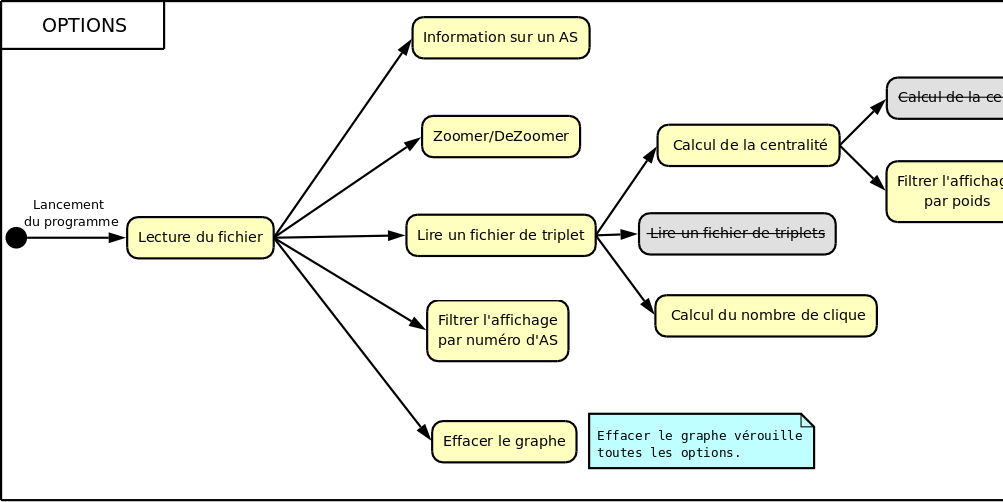
\includegraphics[width=0.8\textwidth]{./schema/seqMenu.png}
  \caption{\label{seq_option}S\'equence du d\'ev\'erouillages des options}
\end{figure}


\subsection{L'exp\'erience utilisateur}
\subparagraph{}
Lors du lancement du programme, l'utilisateur se retrouve devant un fen\^etre o\`u la zone d'affichage est vide et les compteurs de la zone de notification sont tous \`a z\'ero comme c'est le cas sur la figure \ref{ecran_principal}.
\par
\`A ce stade, l'utilisation des options est inutile car elles sont toutes bloqu\'ees en attendant qu'un fichier soit charg\'e produisant un nouveau graphe. L'action du menu \textit{\`A propos} permet d'avoir des informations sur le programme, comme montr\'e figure \ref{ecran_about}.

\begin{figure}[H]
\centering
 \fbox
 {
 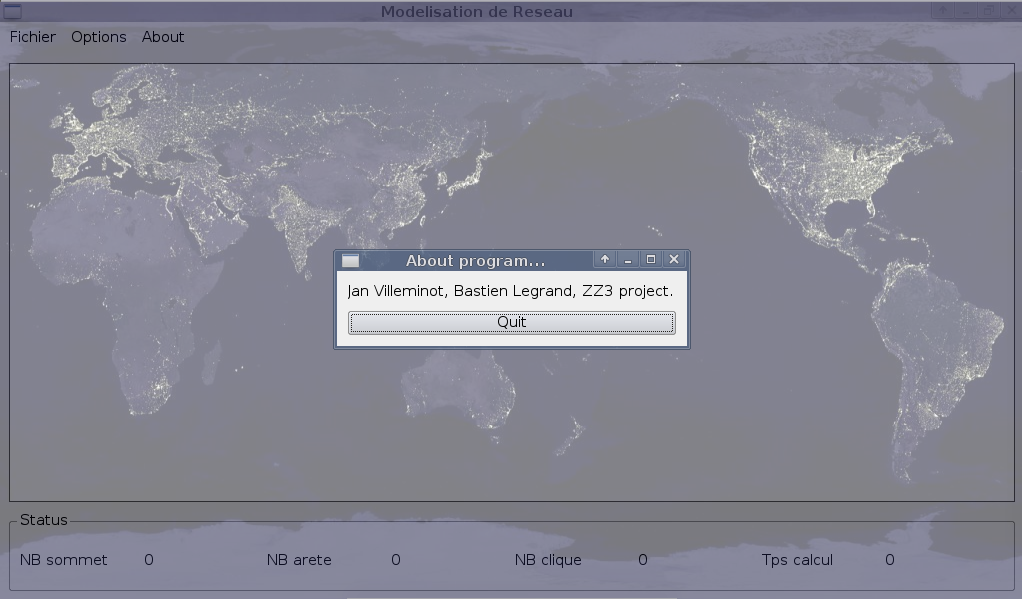
\includegraphics[width=8cm]{./schema/capture_ecran_about.png}
 }
  \caption{\label{ecran_about}Fen\^etre d'informations sur le programme}
\end{figure}

\par
Dans le menu \textit{Fichier}, l'utilisateur a le choix entre ouvrir un fichier de donn\'ees pour construire un graphe ou quitter le programme. Ce menu est illustr\'e figure \ref{ecran_fichier}.

\begin{figure}[H]
\centering
 \fbox
 {
 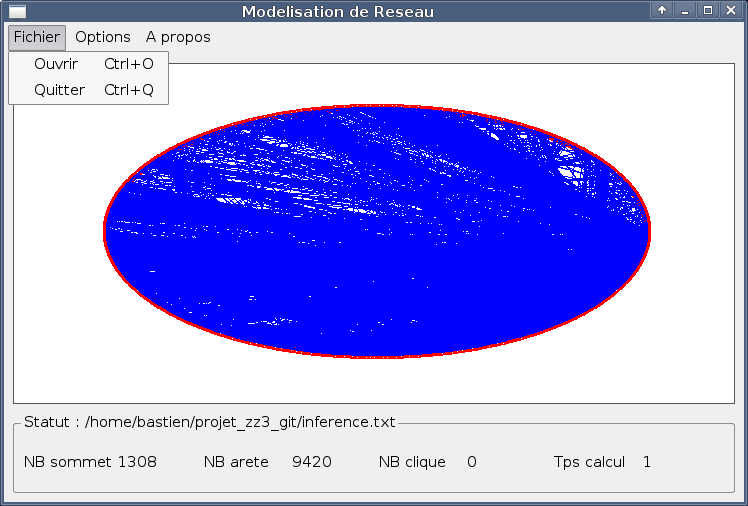
\includegraphics[width=12cm]{./schema/capture_ecran_fichier.png}
 }
  \caption{\label{ecran_fichier}Menu fichier}
\end{figure}

Lorsque l'utilisateur choisit d'ouvrir un fichier de donn\'ees, une nouvelle fen\^etre de navigation s'ouvre et lui demande de choisir son fichier. Il choisit un fichier de donn\'ees \`a ouvrir et le logiciel se charge d'afficher le graphe correspondant en organisant les sommets sur un polyg\^one r\'egulier \`a n c\^ot\'es.
La barre de statut est mise \`a jour avec des informations telles que le nombre de sommets, le nombre d'ar\^etes ou le temps de calcul. Un exemple de graphe est donn\'e figure \ref{ecran_graph}

\begin{figure}[H]
\centering
 \fbox
 {
 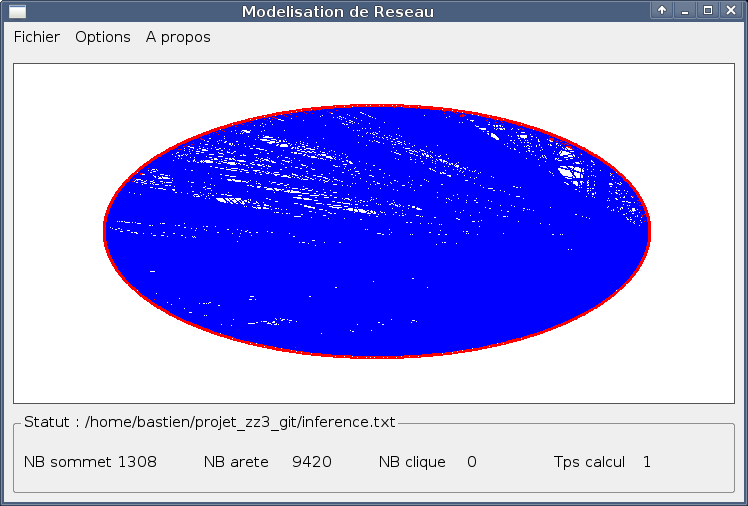
\includegraphics[width=16cm]{./schema/capture_ecran_graph.png}
 }
  \caption{\label{ecran_graph}Ecran principal du programme apr\`es chargement d'un graphe}
\end{figure}

\par
Ensuite, les options d\'ebloqu\'ees lui permettent d'int\'eragir avec le graphe., comme illustr\'e figure \ref{ecran_option}.

\begin{figure}[H]
\centering
 \fbox
 {
 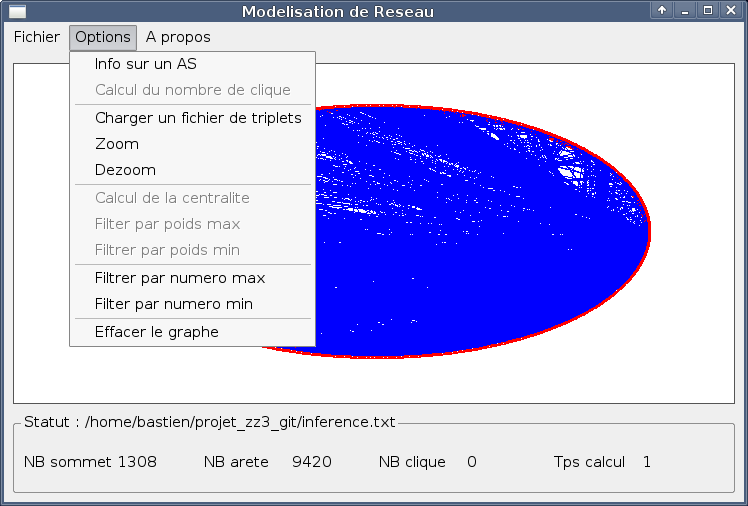
\includegraphics[width=16cm]{./schema/capture_ecran_options.png}
 }
  \caption{\label{ecran_option}Menu des options du programme}
\end{figure}

\subsection{Mise en évidence des caractéristiques d'Internet}
\subparagraph{}
Le programme \'eclaire de fa\c con visuelle certains aspects \'evoqu\'es plus t\^ot dans ce rapport. En effet, on voit au premier chargement d'un fichier que le graphe ressemble \`a un gros ovale bleu, c'est d\^u au grand nombre d'As qui compose Internet et qui rend la repr\'esentation difficile. En comparaison, la structure en IPv6 est clairement plus l\'eg\`ere puisqu'on peut voir du blanc.
\par
Une fois \'elimin\'es les stubs qui ne sont pas pertinents dans le cadre d'une \'etude de topologie du coeur, on peut voir le nombre de clique et on s'apper\c coit qu'en IPv6, il n'y en a qu'une.
\par
Enfin, le calcul de la centralit\'e peut permettre de visualiser plus facilement les ar\^etes sensibles m\^eme si le programme ne dispose pas encore de mode d'affichage sp\'ecifique pour mettre ce point en valeur.
\par
Dans le futur, le logiciel pourra accueillir des ``extensions'' permettant de réaliser de nouveaux traitements sur l'affichage ou les données.